% Created 2024-12-21 Sat 15:05
% Intended LaTeX compiler: pdflatex
\documentclass[11pt]{article}
\usepackage[utf8]{inputenc}
\usepackage[T1]{fontenc}
\usepackage{graphicx}
\usepackage{longtable}
\usepackage{wrapfig}
\usepackage{rotating}
\usepackage[normalem]{ulem}
\usepackage{amsmath}
\usepackage{amssymb}
\usepackage{capt-of}
\usepackage{hyperref}
\usepackage{minted}
\author{Ross}
\date{\today}
\title{}
\hypersetup{
 pdfauthor={Ross},
 pdftitle={},
 pdfkeywords={},
 pdfsubject={},
 pdfcreator={Emacs 29.4 (Org mode 9.8-pre)}, 
 pdflang={English}}
\begin{document}

\begin{center}
\begin{tabular}{lllllll}
\href{assignments.html}{Assignments} & \href{contact.html}{Contact} & \href{index.html}{Index} & \href{projects.html}{Projects} & \href{work\_experience.html}{WorkExperience} & \href{cv/rossMikulskisResume.pdf}{CV} & \href{research/index.html}{Research/}\\
\end{tabular}
\end{center}
\section*{Ross A. Mikulskis}
\label{sec:org3af4158}

\begin{center}
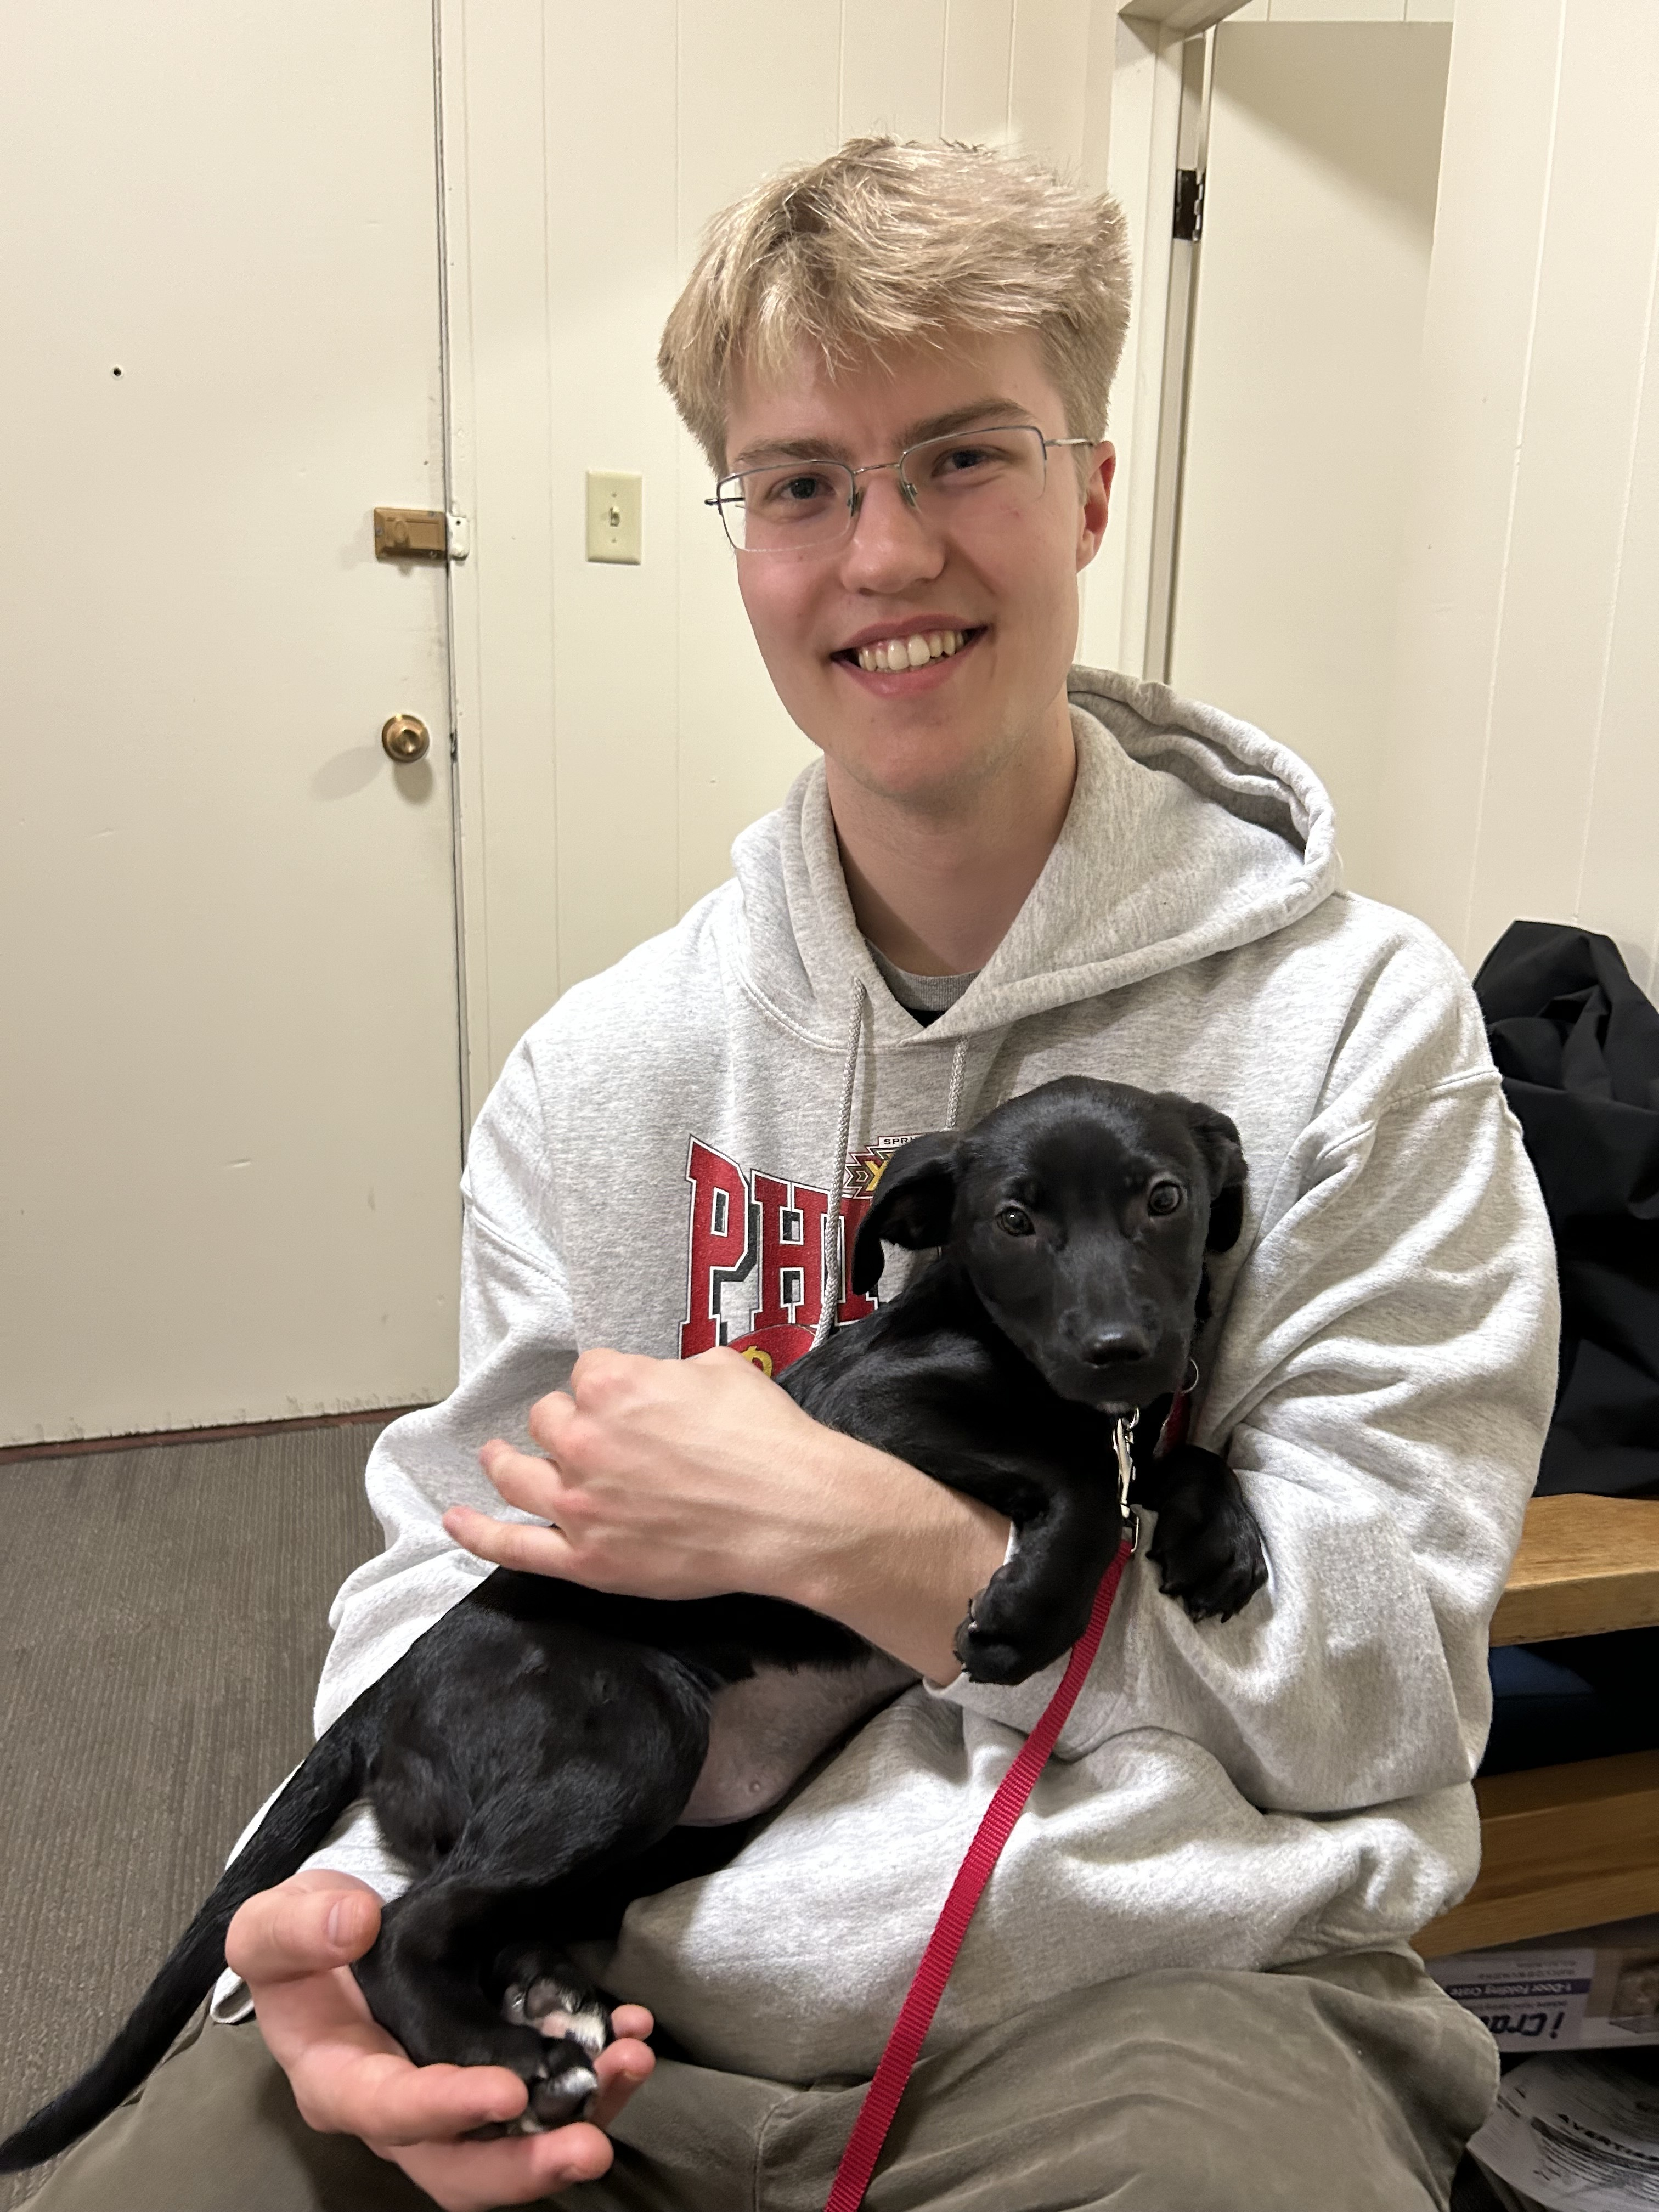
\includegraphics[width=.9\linewidth]{./profile.jpg}
\end{center}

\href{https://bitsofcs.com/}{Bits of CS (my computer science textbook)}

Hello! My name is Ross, I am a senior at Boston University studying
computer science. I'm in my final year of the BA/MS, so I will be completing
my master's along with my bachelor's in May of 2025.

I love operating systems, my favorite things to use are Emacs and C. I also
dabble in cloud engineering (e.g. Kubernetes, CI/CD). I will be
applying to PhD programs this fall and hope to become Dr. Ross in the near future!

Outside of computer science, I play the trumpet in the New Jazz Orchestra
around Cambridge, MA. I also have been a big brother in the Boston Big Brothers
Big Sisters program for the past year. I have a dog named Winnie (picture above),
and I'm a proud brother of Phi Kappa Tau. 
\end{document}
